\subsection{Evolution from MobileNet to EfficientNet}
The network optimisation strategy for CNN models is covered in the evolution process of MobileNet and EfficientNet. This subsection will introduce vital ideas and innovations proposed by each version.

\citet{howard2017mobilenets} proposed a lightweight convolutional neural network focused on mobile devices, namely MobileNet.
The first version of the proposed model uses sequential convolutional layered architecture like VGG but replaces standard convolutions with depthwise separable convolutions to greatly reduce the calculations required in convolutions.

\begin{figure}[!ht]
    \centering
    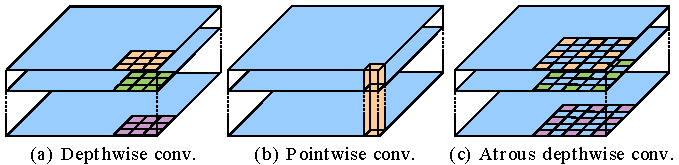
\includegraphics[width=.8\textwidth]{literature/imgs/ext-2-mobile-depth-point-atrous.pdf}
    \caption{Depthwise, pointwise and atrous convolution \cite{chen2018encoder}}
    \label{fig:ext-2-mobile-depth-point-atrous}
\end{figure}

The depthwise separable convolution splits the standard convolution into two operations, depthwise convolution (Figure \ref{fig:ext-2-mobile-depth-point-atrous} (a)) and pointwise convolution (Figure \ref{fig:ext-2-mobile-depth-point-atrous} (b)) respectively.
In detail, Formula \ref{equ:2-standard-conv} expresses the calculation of standard convolution, and it has the computational cost of $D_K \cdot D_K \cdot M \cdot N \cdot D_F \cdot D_F$, where $M$ and $N$ denote the number of input and output channels; $D_K$ and $D_F$ denote the dimension of kernels and feature maps.

\begin{minipage}[!ht]{.48\textwidth}
\begin{equation}
    \mathbf{G}_{k, l, n}=\sum_{i, j, m} \mathbf{K}_{i, j, m, n} \cdot \mathbf{F}_{k+i-1, l+j-1, m}
    \eqcite{howard2017mobilenets}
    \label{equ:2-standard-conv}
\end{equation}
\end{minipage}
\begin{minipage}[!ht]{.48\textwidth}
\begin{equation}
    \hat{\mathbf{G}}_{k, l, m}=\sum_{i, j} \hat{\mathbf{K}}_{i, j, m} \cdot \mathbf{F}_{k+i-1, l+j-1, m}
    \eqcite{howard2017mobilenets}
    \label{equ:2-depthwise-conv}
\end{equation}
\end{minipage}

Formula \ref{equ:2-depthwise-conv} shows that depthwise convolution uses only one convolution kernel for each channel, and there is one to one map from each input channel to each output channel, thus the computational cost is $D_K \cdot D_K \cdot M \cdot D_F \cdot D_F$.
The pointwise convolution is a standard convolution with kernel size of $1\times1$ that perform a combination of the inputs along the channel direction, so the computational cost is $M \cdot N \cdot D_F \cdot D_F$.
By comparing computational cost formulae, total deduction for depthwise separable convolution is $\frac{1}{N}+\frac{1}{D_{K}^{2}}$.

\begin{figure}[!ht]
    \centering
    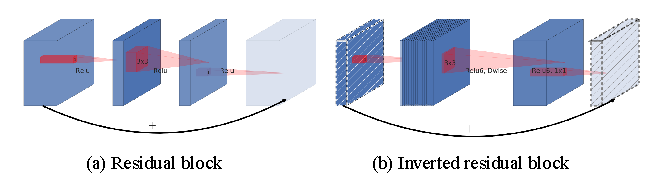
\includegraphics[width=.85\textwidth]{literature/imgs/ext-inverted-residual.pdf}
    \caption{Compare residual block and inverted residual block \cite{sandler2018mobilenetv2}}
    \label{fig:ext-inverted-residual}
\end{figure}

One year after the release of the first version of MobileNet, \citet{sandler2018mobilenetv2} contributed two new ideas in the second version to further optimise the performance of the MobileNet model.
The first one is the inverted residual building block shown in Figure \ref{fig:ext-inverted-residual} (b).
As compared in the figure, the original residual design in ResNet (Figure \ref{fig:ext-inverted-residual} (a)) reduce dimension first and extraction with standard convolution, but in inverted residual design, the dimension is increased first and use depthwise convolution in the middle.
The second alternation is using a linear bottleneck in the last layer in each inverted residual building block to avoid feature information lost in non-linear activation, especially for Rectified Linear Unit (ReLU) that always outputs zero gradients for any neuron weights zero (dead neuron).

In 2019, \citet{tan2020efficientnet} proposed EfficientNet that inherited the design ideas from MobileNetV2 with a systematical methodology to scale up the model in network depth, width and input resolution to obtain better balance between accuracy and efficiency.
Figure \ref{fig:ext-efficientnetb0} illustrates the architecture of the proposed baseline network EfficientNet-B0.
The network is mainly composed of mobile inverted bottleneck convolution(MBConv) proposed in MobileNetV2.
The result shows that it achieves a Top-1 accuracy of 77.1\% on ImageNet with 5.3M parameters and 0.39B Flops.

\begin{figure}[!ht]
    \centering
    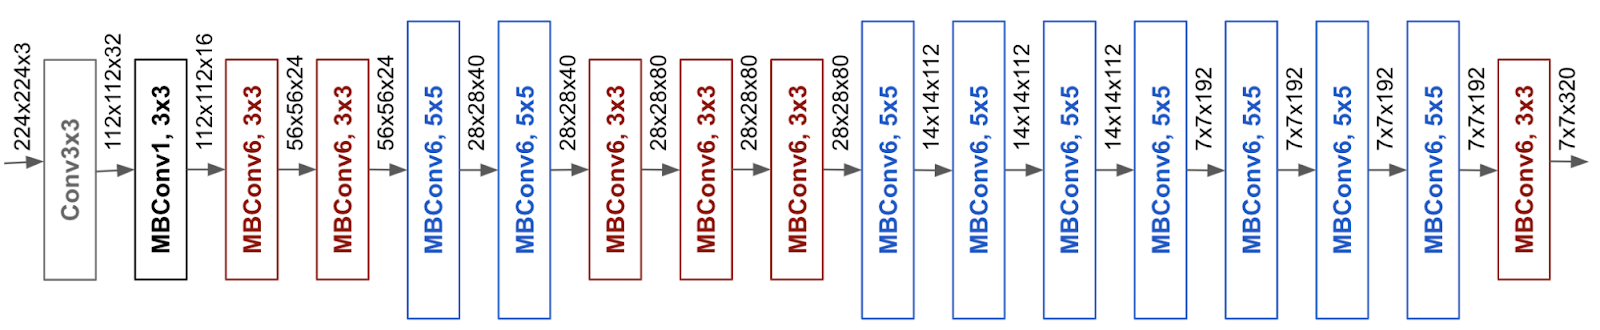
\includegraphics[width=\textwidth]{literature/imgs/ext-efficientnetb0.png}
    \caption{The architecture of baseline network EfficientNet-B0 \cite{tan2020efficientnet}}
    \label{fig:ext-efficientnetb0}
\end{figure}

Two years after the debut of EfficientNet, \citet{tan2021efficientnetv2} proposed the second version of EfficientNet in 2021, which has a smaller model and faster training and achieves state-of-the-art results on ImageNet.
